% !TEX root = saveliev_physics_general_course_1.tex
%!TEX TS-program = pdflatex
%!TEX encoding = UTF-8 Unicode

\chapter{PHYSICAL KINETICS}\label{chap:16}

\section{Transport Phenomena}\label{sec:16_1}

Statistical physics has to do with equilibrium states and reversible processes (\ie, processes in which a system passes through a sequence of equilibrium states). The science studying the processes that are set up when equilibrium is violated is called \textbf{physical kinetics}.

When equilibrium of a system is violated, the system tends to return to its equilibrium state. This process is attended by a growth in entropy and is consequently irreversible. Thus, the processes which physical kinetics studies are irreversible.

The violation of equilibrium is accompanied by the appearance of flows of either molecules, or heat, or an electric charge, and so on. In this connection, the relevant processes are called \textbf{transport phenomena}. It follows from the above that transport phenomena are irreversible processes.

We shall consider three transport phenomena---diffusion, thermal conductivity, and internal friction or viscosity. We shall deal only with the cases when deviations from equilibrium are not considerable. First, we shall write empirical equations of these processes applicable to any media (solid, liquid, and gaseous). In the following sections, we shall give the molecular-kinetic derivation of these equations for gases.

When considering transport phenomena, we shall have to calculate the amounts of various quantities (the number of particles, mass, energy, momentum) transported through an imaginary surface. The amount of a quantity passing in unit time through a surface is called the \textbf{flux} (\textbf{flow}) of this quantity. Examples are the flux (flow) of a liquid through a cross section of a pipe or tube, and the light flux through a window pane or through the glass bulb of an electric lamp. We can consider the flux through a surface of any shape; in particular, the surface can be closed.

The flux is a scalar algebraic quantity. The sign of a flux is determined by the choice of the positive direction, for example, the direction of the axis along which the flux propagates. The positive direction is usually chosen arbitrarily. For closed surfaces, it is customary practice to consider the flux flowing out of the surface as positive, and that flowing into it as negative. In this chapter, we shall deal with fluxes through flat surfaces perpendicular to the $z$-axis. If particles, energy, or momentum will be transported through the surface in the direction of the $z$-axis, we shall consider the corresponding flux to be positive, otherwise we shall consider it negative.

Every transport phenomenon is due to changes in a certain quantity $f$ in space. This quantity for the transport of particles (diffusion) is the concentration of the particles---the latter are transported in the direction of diminishing of their concentration. A heat flux appears when the temperature at different points of the medium differs, the heat flowing in the direction of diminishing temperature, etc.

We shall consider for simplicity that the quantity $f$ whose lack of homogeneity underlies the given transport process (the concentration, temperature, etc.) is a function of only the coordinate $z$. Hence, the change in this quantity in space will he characterized by the derivative $\diffin{f}{z}$. The latter is usually called the gradient of the quantity $f$. This name is not quite correct---strictly speaking, the derivative of the scalar function $f=f(z)$ with respect to $z$ gives the projection of the gradient of the function onto the $z$-axis [see \eqn{3_23}]. Following the tradition, however, we shall call quantities of the kind $\diffin{f}{z}$ in a transport equation a \textbf{gradient}.

\textbf{Diffusion.} Diffusion is defined as the spontaneous levelling out of the concentrations in a mixture of several (in the simplest case of two) different substances due to thermal motion. This process is observed in solid, liquid, and gaseous media. We shall consider only gaseous media.

Assume that a unit volume of a two-component gas mixture contains $n_1$ molecules of one species and $n_2$ molecules of another one. The total number of molecules in unit volume is $n=n_1+n_2$. The ratio
\begin{equation*}
    c_i = \frac{n_i}{n}
\end{equation*}

\noindent
is called the \textbf{relative concentration} of the molecules of the $i$-th species.

\begin{figure}[t]
	\begin{center}
		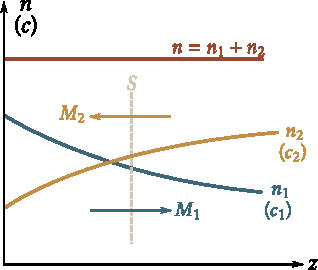
\includegraphics[scale=1]{figures/ch_16/fig_16_1.pdf}
		\caption[]{}
		\label{fig:16_1}
	\end{center}
	\vspace{-0.8cm}
\end{figure}

Let us assume that concentration gradients $\diffin{c_1}{z}$ and $\diffin{c_2}{z}$ are set up in the direction of the $z$-axis, and $\diffin{c_1}{z}=-\diffin{c_2}{z}$ (\fig{16_1}). Hence,
\begin{equation*}
    \frac{\upd}{\deriv{z}}(c_1 + c_2) = \frac{1}{n}\frac{\upd}{\deriv{z}}(n_1 + n_2) = 0
\end{equation*}

\noindent
so that $n$ and, consequently, $p$ are constant ($p=nkT$). Therefore, no gas-dynamical fluxes appear. But owing to the thermal motion of the molecules, the process of levelling out of the concentrations will occur attended by the transport of the mass of each of the components in the direction of the diminishing of its concentration. As indicated above, this process is called diffusion.

It has been established experimentally that the flux of molecules of the $i$-th species through surface $S$ perpendicular to the $z$-axis is determined by the expression
\begin{equation}\label{eq:16_1}
    N_i = -D \diff{n_i}{z} S
\end{equation}

\noindent
where $D$ is a constant of proportionality called the \textbf{diffusion coefficient}.

According to \eqn{16_1}, when $\diffin{n_i}{z}>0$, the flux $N_i$ is negative; this signifies that the molecules are transported in a direction opposite to that of the $z$-axis (\fig{16_2}a). When $\diffin{n_i}{z}<0$, the flux is positive, \ie, the molecules are transported in the direction of the $z$-axis (\fig{16_2}b). Thus, the minus sign in \eqn{16_2} is due to the fact that the molecules flow in the direction of diminishing of the concentration.

The dimension of the flux of molecules $N$ is T$^{-1}$, that of $n_i$ is L$^{3}$, of the area $S$ is L$^{2}$, and $\deriv{z}$ has the dimension L. Hence, the diffusion coefficient has the dimension L$^2$T$^{-1}$. Multiplying both sides of \eqn{16_1} by the mass of a molecule of the $i$-the species $m_i$ we get an expression for the flux of the mass of the $i$-th component:
\begin{equation}\label{eq:16_2}
    M_i = -D \diff{\rho_i}{z} S.
\end{equation}

\noindent
Here $\rho_i=n_im_i$ is the partial density of the $i$-th component; it is also called the \textbf{absolute concentration}.

Equations~\eqref{eq:16_1} and~\eqref{eq:16_2} are empirical equations of diffusion. They are also called \textbf{Fick's law}.

\begin{figure}[t]
	\begin{center}
		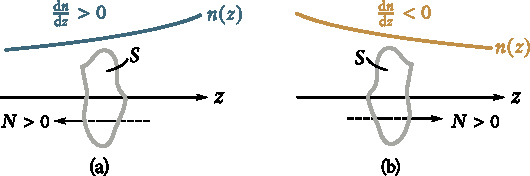
\includegraphics[scale=1]{figures/ch_16/fig_16_2.pdf}
		\caption[]{}
		\label{fig:16_2}
	\end{center}
	\vspace{-0.8cm}
\end{figure}

\textbf{Thermal Conductivity.} Experiments show that if we set up a temperature gradient along the $z$-axis in a medium (solid, liquid, or gaseous one), then a heat flux is produced whose magnitude is determined by the formula
\begin{equation}\label{eq:16_3}
    q = -\varkappa \diff{T}{z} S
\end{equation}

\noindent
where $q$ is the heat flux through surface $S$ perpendicular to the $z$-axis, $\diffin{T}{z}$ is the temperature gradient (more exactly, the projection of the temperature gradient on the $z$-axis) and $\varkappa$ is a proportionality constant depending on the properties of the medium and called the \textbf{thermal conductivity coefficient}.

The unit of $q$ is \si{\joule\per\second}, \ie, \si{\watt} (watt). Hence, $\varkappa$ is measured in watts per metre-kelvin $\bracket{\si{\watt\per\metre\per\kelvin}}$. The minus sign in \eqn{16_3} signifies
that the heat flows in the direction of diminishing of the temperature. Therefore, the signs of $q$ and $\diffin{T}{z}$ are opposite. Equation~\eqref{eq:16_3} is an empirical equation of thermal conductivity. It is also called the \textbf{Fourier law}.

\textbf{Internal Friction.} According to \eqn{9_12}, the force of friction between two layers of a fluid is
\begin{equation}\label{eq:16_4}
    F = \eta \absolute{\diff{u}{z}} S
\end{equation}

\noindent
where $\eta$ is the viscosity (viscosity coefficient), $\diffin{u}{z}$ is the quantity showing how rapidly the velocity of the fluid changes in the direction $z$ perpendicular to the direction of motion of the layers (the gradient of $u$) and $S$ is the surface area over which the force $F$ acts.

Equation~\eqref{eq:16_4} is the empirical equation of viscosity.

According to Newton's second law, the interaction of two layers with the force $F$ can be considered as a process in the course of which a momentum equal to $F$ in magnitude is transmitted from one layer to another in unit time. Therefore, \eqn{16_4} can be written in the form
\begin{equation}\label{eq:16_5}
    K = -\eta \diff{u}{z} S
\end{equation}

\noindent
where $K$ is the momentum transmitted in one second from layer to layer through surface $S$, \ie, the momentum flux through $S$.

The momentum flux $K$ is measured in \si{\kilo\gram\metre\per\second\squared}. Hence, the unit of the viscosity $\eta$ is the kilogramme per metre-second $\bracket{[\si{\kilo\gram\per\metre\per\second}}$. [This unit can also be written in the form pascal-second (\si{\pascal\second}).]

The minus sign in \eqn{16_5} is due to the circumstance that the momentum ``flows'' in the direction of the decrease in the velocity $u$. Therefore, the signs of the flux $K$ and of the derivative $\diffin{u}{z}$ are opposite.

It must be remembered that \eqn{16_4} determines the identical modulus of two oppositely directed forces with which the layers act on each other. Therefore, the minus sign must not be written in front of the right-hand side of \eqn{16_4}. In addition, we must take the magnitude of the expression $\diffin{u}{z}$ (the magnitude of the force with any sign of the derivative $\diffin{u}{z}$ must be positive).

\section{Mean Free Path}\label{sec:16_2}

The molecules of a gas in thermal motion continuously collide with one another. The term ``collision'' as applied to molecules must not be understood literally and the process conceived as the collision of rigid balls. By a collision of molecules is meant the process of interaction
between them as a result of which the molecules change the direction of their motion.

\begin{figure}[t]
	\begin{center}
		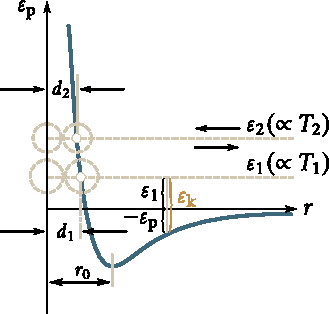
\includegraphics[scale=1]{figures/ch_16/fig_16_3.pdf}
		\caption[]{}
		\label{fig:16_3}
	\end{center}
	\vspace{-0.8cm}
\end{figure}

Figure~\ref{fig:16_3} shows a curve depicting the mutual potential energy of two molecules as a function of the distance $r$ between their
centres. Let us use this curve to consider the process of the approach (collision) of molecules. Let us mentally place the centre of one of the molecules at the origin of coordinates, and imagine the centre of the second molecule moving along the $r$-axis. Assume that the second molecule is flying toward the first one from infinity having the initial store of kinetic energy $\ab{\varepsilon}{k}=\varepsilon_1$. Approaching the first molecule, the second one under the action of the force of attraction moves with a constantly growing velocity. The kinetic energy of a molecule $\ab{\varepsilon}{k}$ also grows as a result. The total energy of the system equal to $\varepsilon=\ab{\varepsilon}{k}+\ab{\varepsilon}{p}$, however, remains unchanged (the system of the two molecules is closed) and equal to $\varepsilon_1$ because the potential energy $\ab{\varepsilon}{p}$ diminishes simultaneously. When the molecule passes the point with the coordinate $r_0$, the forces of attraction are replaced by forces of repulsion, owing to which the molecule begins to rapidly lose its velocity (in the region of repulsion the curve of $\ab{\varepsilon}{p}$ is very steep).
At the moment when the potential energy $\ab{\varepsilon}{p}$ becomes equal to the total energy of the system $\varepsilon_1$, the velocity of the molecule vanishes. At this moment, the molecules approach each other to the closest distance. After the molecule stops, all the phenomena proceed in the reverse sequence: first the molecule travels with a constantly growing velocity under the action of the force of repulsion, upon covering the distance $r_0$, the molecule gets under the action of the force of attraction that retards its motion and, finally, travels away to infinity having its initial store of kinetic energy $\varepsilon_1$.

The minimum distance between the centres of two molecules when they collide is called the \textbf{effective} or \textbf{collision diameter} of a molecule $d$ (\fig{16_4}). The quantity
\begin{equation}\label{eq:16_6}
    \sigma = \pi d^2
\end{equation}

\noindent
is known as the effective section of a molecule.

\begin{figure}[t]
	\begin{center}
		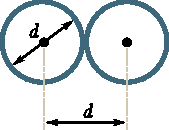
\includegraphics[scale=1]{figures/ch_16/fig_16_4.pdf}
		\caption[]{}
		\label{fig:16_4}
	\end{center}
	\vspace{-0.8cm}
\end{figure}

A glance at \fig{16_3} shows that when a molecule begins its motion from infinity with a greater store of energy, the minimum distance between the centres of the molecules when they approach is less (compare $d_1$ and $d_2$ in the figure). Thus, the collision diameter of molecules depends on their energy and, consequently, on the temperature. The collision diameter of molecules diminishes with increasing temperature.

During one second, a molecule travels an average path equal to the mean velocity $\average{v}$. If it experiences an average of $\nu$ collisions a second, then the mean free path will be
\begin{equation}\label{eq:16_7}
    l = \frac{\average{v}}{\nu}.
\end{equation}

To calculate the average number of collisions $\nu$, let us first assume that all the molecules except for a given one are frozen still in their places. Let us watch the motion of the molecule we have earmarked. After striking one of the stationary molecules, it will fly in a straight line until it collides with another stationary molecule (\fig{16_5}). This collision will occur if the centre of the stationary molecule is at a distance from the line of flight of the molecule less than the collision diameter of a molecule $d$. As a result of the collision, the molecule will change the direction of its motion, and will then again fly along a straight line for a time. This will continue until it encounters another molecule whose centre will be within the cylinder of radius $d$ shown in \fig{16_5}.

The molecule travels a path of $\average{v}$ in one second. The number of collisions with stationary molecules occurring during this time equals the number of molecules whose centres are within the bent cylinder of length $\average{v}$ and radius $d$. It will be shown below that the mean free path is much larger than the collision diameter of the molecules $d$. Therefore, the volume of the cylinder can be considered equal to $\pi d^2\average{v}$. Multiplying this volume by the number of molecules in a unit volume $n$, we get the average number of collisions of a moving molecule with stationary ones per second:
\begin{equation}\label{eq:16_8}
    \nu' = \pi d^2 \average{v} n.
\end{equation}

\begin{figure}[t]
	\begin{center}
		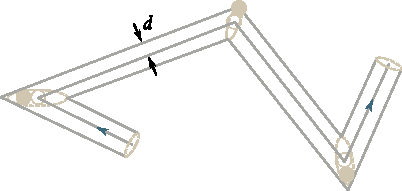
\includegraphics[scale=1]{figures/ch_16/fig_16_5.pdf}
		\caption[]{}
		\label{fig:16_5}
	\end{center}
	\vspace{-0.8cm}
\end{figure}

Actually, all the molecules are in motion, owing to which the number of collisions is determined by the mean velocity of motion of the molecules with respect to one another, and not by the mean velocity $\average{v}$ of molecules relative to the walls of the vessel confining them. The relative velocity of two arbitrarily taken molecules is
\vspace{-12pt}
\begin{equation*}
    \ab{\vec{v}}{rel} = \vec{v}_2 - \vec{v}_1.
\end{equation*}

\noindent
Squaring this equation, we get
\begin{equation*}
    \ab{v}{rel}^2 = \parenthesis{\vec{v}_2 - \vec{v}_1}^2 = v_2^2 + v_1^2 - 2\vec{v}_1\vec{v}_2
\end{equation*}

\noindent
(we have taken advantage of the fact that $\vec{v}^2=v^2$). The mean value of the sum of several quantities equals the sum of the mean values of the quantities being added. Hence,
\begin{equation*}
    \average{\ab{v}{rel}^2} = \average{v_2^2} + \average{v_1^2} - 2\average{\vec{v}_1\vec{v}_2}.
\end{equation*}

\noindent
Events consisting in that a first molecule has the velocity $\vec{v}_1$ and a second one the velocity $\vec{v}_2$ are statistically independent. Therefore, $\average{\vec{v}_1\vec{v}_2}=\average{\vec{v}_1}\average{\vec{v}_2}$. Each of the multipliers equals zero for a gas in equilibrium. Thus,
\begin{equation*}
    \average{\ab{v}{rel}^2} = \average{v_2^2} + \average{v_1^2} = 2\average{v^2}
\end{equation*}

\noindent
(the mean value of the square of the velocity of all the molecules is the same and equals $\average{v^2}$). The result obtained signifies that $\ab{v}{rel,m. sq}=\sqrt{2}\ab{v}{m. sq}$. The mean square velocities are proportional to the arithmetical mean ones. Consequently,
\begin{equation*}
    \average{\ab{v}{rel}} = \sqrt{2}\average{v}.
\end{equation*}

Substituting $\average{\ab{v}{rel}}$ for $\average{v}$ in \eqn{16_8}, we get the following expression for the mean number of collisions:
\begin{equation}\label{eq:16_9}
    \nu = \sqrt{2}\pi d^2 \average{v} n.
\end{equation}

\noindent
Using this value of $\nu$ in \eqn{16_7}, we get the following equation for the mean free path:
\begin{equation}\label{eq:16_10}
    l = \frac{1}{\sqrt{2}\pi d^2 n}.
\end{equation}

\noindent
Substituting $\sigma$ for $\pi d^2$ in the above equation in accordance with \eqn{16_6}, we get
\begin{equation}\label{eq:16_11}
    l = \frac{1}{\sqrt{2}\sigma n}.
\end{equation}

At constant temperature, $n$ is proportional to $p$. Hence, the mean free path is inversely proportional to the pressure:
\begin{equation}\label{eq:16_12}
    l \propto \frac{1}{p}.
\end{equation}

\noindent
We noted above that the collision diameter of molecules diminishes with increasing temperature. Accordingly, elevation of the temperature is attended by an increase in the free path.

Let us assess the value of the mean free path and the average number of collisions a second. We established in \sect{10_2} that molecules have dimensions of the order of several angstroms. Let us adopt the collision diameter of a molecule equal to \SI{2}{\angstrom}, \ie, \SI{2e-10}{\metre}. A mole of a gas in standard conditions (\ie, at \SI{0}{\degreeCelsius} and $p=\SI{1}{\atm}$) occupies a volume of \SI{22.4e-3}{\metre\cubed}. The number of molecules in unit volume in these conditions is $\num{6e23}/\num{22.4e-3}\approx\SI{3e25}{\per\metre\cubed}$. Introducing these numbers into \eqn{16_10}, we have
\begin{equation*}
    l = \frac{1}{\sqrt{2}\times 3.14\times \num{4e-20}\times\num{3e25}} \approx \SI{2e-7}{\metre} = \SI{2e-5}{\centi\metre}.
\end{equation*}

At a pressure of \SI{e-3}{\mmHg} (which corresponds to about \SI{e-6}{\atm}), $l$ will be of the order of \SI{10}{\centi\metre}. If a vessel has dimensions of a few centimetres, then at such a pressure the molecules will travel from wall to wall virtually without colliding with one another. At a pressure of \SI{e-6}{\mmHg} $l$ reaches a value of scores of metres.

When deriving \eqn{16_8}, we assumed that $l$ is much greater than $d$. Now we can see that this assumption is correct. Indeed, it follows from the above assessment that in standard conditions the ratio of $l$ to $d$ is about $\num{2e-5}/\num{2e-10} = \num{e5}$.

We can find the number of collisions a second by dividing the mean velocity of the molecules $\average{v}$ by $l$. In \sect{11_6}, we obtained a value of $\average{v}$ of about \SI{500}{\metre\per\second} for oxygen. Dividing this value by $l=\SI{2e-7}{\metre}$, we get a value of \SI{2.5e9}{\per\second} for the number of collisions a second. Thus, in standard conditions, the number of collisions a second is several thousand millions. The number of collisions diminishes with a decreasing pressure, changing in proportion to $p$ [see \eqn{16_12}].

\section{Diffusion in Gases}\label{sec:16_3}

We shall attempt to get an equation of diffusion proceeding from molecular-kinetic notions. To simplify our task, we shall consider that the molecules of both components differ only slightly in mass ($m_1\approx m_2\approx m$) and have virtually identical effective sections ($\sigma_1\approx\sigma_2\approx\sigma$). In this case, we
can assign the same mean velocity of thermal motion $\average{v}$ to the molecules of both components and calculate the mean free path by the equation
\begin{equation*}
    l = \frac{1}{\sqrt{2}\sigma n}
\end{equation*}

\noindent
where $n=n_1+n_2$.

It is easy to understand that the process of diffusion in gases will proceed more intensively when the molecules have a higher velocity $\average{v}$ and collide less frequently with one another (\ie, the free path $l$ is greater). Consequently, we can expect that the diffusion coefficient $D$ must be proportional to the product $\average{v}l$. This agrees with the fact that, as we noted in \sect{16_1}, the dimension of $D$ is L$^2$T$^{-1}$.

\begin{figure}[t]
	\begin{center}
		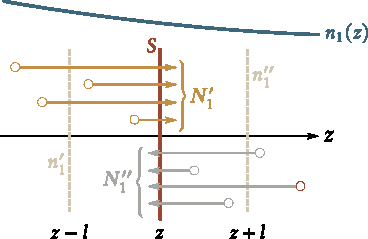
\includegraphics[scale=1]{figures/ch_16/fig_16_6.pdf}
		\caption[]{}
		\label{fig:16_6}
	\end{center}
	\vspace{-0.8cm}
\end{figure}

Let us begin our calculations. Assume that the change in the concentration of the first component along the $z$-axis is described by the function $n_1=n_1(z)$. Let us denote the number of molecules of the first component flying through area $S$ in the direction of the $z$-axis a second by $N_1'$, and the number of molecules flying in the direction opposite to the $z$-axis by $N_1''$ (\fig{16_6})\footnote{We have drawn \fig{16_6} so that the molecules $N_1'$ fly through the upper half and the molecules $N_1''$ through the lower half of area $S$. Actually, both groups of molecules are distributed over the entire surface $S$.}. The difference between these numbers is the flux of the molecules of the first component $N_1$ through surface $S$:
\begin{equation}\label{eq:16_13}
    N_1 = N_1' - N_1''.
\end{equation}

We shall proceed from the simplified notion according to which the molecules move along three mutually perpendicular directions coinciding with the axes $x, y, z$ (the axes $x$ and $y$ are parallel to area $S$). In this case according to \eqn{11_24}, the number of molecules flying one of the directions through unit area a second is $n\average{v}/6$. Hence, the numbers $N_1'$ and $N_1''$ can be represented in the form
\begin{equation}\label{eq:16_14}
    N_1' = \frac{1}{6}n_1'\average{v} S,\quad N_1'' = \frac{1}{6}n_1''\average{v} S.
\end{equation}

\noindent
where $n_1'$ is the ``effective'' concentration of the molecules of the first component to the left of $S$, $n_1''$ is the same to the right of $S$.

Molecules will fly through surface $S$ that experienced their last collision at different distances from it. On an average, however, the last collision will occur at a distance from $S$ equal to the mean free path $l$. It is therefore reasonable to take the value $n_1(z-l)$ as $n_1'$, and $n_1(z+l)$ as $n_1''$ (see \fig{16_6}). Hence, with a view to Eqs.~\eqref{eq:16_13} and~\eqref{eq:16_14}, we can write that
\begin{equation}\label{eq:16_15}
    N_1 = \frac{1}{6}\average{v} S [n_1(z-l) - n_1(z+l)].
\end{equation}

Since $l$ is very small, the difference between the values of the function $n_1(z)$ given in \eqn{16_15} in brackets can be written in the
form\footnote{Equation~\eqref{eq:16_16} holds provided that the change in $n_1$ over the free path is much smaller than $n_1$ itself $(\diffin{n_1}{z}l\leqslant n_1)$. This condition gives a criterion for the smallness of the deviation from equilibrium (see the fourth paragraph of \sect{16_1}). This remark relates to similar formulas of the following two sections. For example, \eqn{16_23} holds provided that $\diffin{T}{z}l\leqslant T$.}
\begin{equation}\label{eq:16_16}
    n_1(z-l) - n_1(z+l) = - \diff{n_1}{z}2l.
\end{equation}

\noindent
Introducing this expression into \eqn{16_15}, we find that
\begin{equation}\label{eq:16_17}
    N_1 = - \parenthesis{\frac{1}{3} \average{v} l}\diff{n_1}{z} S.
\end{equation}

A comparison of Eqs.~\eqref{eq:16_1} and~\eqref{eq:16_17} shows that on the basis of molecular-kinetic notions we can not only arrive at a proper dependence of $N_1$ on $\diffin{n_1}{z}$, but also obtain an expression for the diffusion coefficient $D$. This expression has the form
\begin{equation}\label{eq:16_18}
    D = \frac{1}{3} \average{v} l.
\end{equation}

\noindent
More strict calculations lead to the same formula, but with a somewhat different numerical factor.

It must be noted that as we assumed, the diffusion coefficient is proportional to the product $\average{v}l$.

The derivation that led us to \eqn{16_17} can be applied with equal rights to both components of a mixture. Hence, the diffusion coefficient has the same value for both components.

Let us investigate the expression we have obtained for the diffusion coefficient $D$. Inserting in \eqn{16_18} the expressions for $\average{v}$ and $l$, we find that
\begin{equation}\label{eq:16_19}
    D \propto \frac{1}{n\sigma} \parenthesis{\frac{T}{m}}^{1/2}.
\end{equation}

\noindent
It follows from \eqn{16_9} that the diffusion coefficient is inversely proportional to the number of molecules in a unit volume, and, consequently, to the pressure $p$:
\begin{equation*}
    D \propto \frac{1}{p}.
\end{equation*}

\noindent
With elevation of the temperature, $D$ grows approximately in proportion to $\sqrt{T}$ (we remind our reader that $\sigma$ slightly depends on $T$).

We have assumed that the molecules of both components are identical in mass and effective section. Therefore, \eqn{16_18} is in essence an expression for the coefficient of self-diffusion, \ie, the diffusion of the molecules of a gas in a medium containing molecules of the same gas. The phenomenon of self-diffusion could be observed if we marked in some way or other part of the molecules of a homogeneous gas. If the concentrations of marked molecules and of the molecules bearing no marks were not constant, counterflows of the two kinds of molecules would appear in the gas, and the magnitude of the flows would be determined by \eqn{16_17}. Self-diffusion can be studied in practice by employing the tracer technique. It consists in using a mixture of isotopes, \ie, varieties of atoms of the same element differing from each other, for example, in that one variety of the atoms is radioactive and the other is stable.

When the molecules of the two components of a mixture differ in their mass and in effective section, the diffusion coefficient is determined by the expression
\begin{equation*}
    D = \frac{n_1\average{v_2}l_2 + n_2\average{v_1}l_1}{3\parenthesis{n_1 + n_2}}
\end{equation*}

\noindent
where $n_1, \average{v_1}, l_1$ are the concentration, mean velocity and mean free path of the molecules of the first component, and $n_2, \average{v_2}, l_2$ represent the same quantities for the molecules of the second component.

\section{Thermal Conductivity of Gases}\label{sec:16_4}

Let us calculate the heat flux in a gas on the basis of molecular-kinetic notions. If the temperature of the gas differs at different points, then the mean energy of the molecules at these points will also differ. Being displaced owing to thermal motion from one set of points to another, the molecules transport the energy they have stored. This energy transfer underlies the process of thermal conductivity in gases. Before beginning our calculations, let us attempt to reveal the factors that can affect the ability of a gas to conduct heat. It is easy to understand that apart from the factors determining the rate of diffusion, \ie, the mean velocity of the molecules $\average{v}$ and
the free path $l$, the amount of energy transported by the molecules must depend on the ability of the molecules to store energy, \ie, on the heat capacity of the gas.

Let us consider a gas in which a temperature gradient is maintained in some way or other along the direction which we have denoted by the letter $z$. Let us mentally imagine area $S$ perpendicular to this direction (\fig{16_7}).

\begin{figure}[t]
	\begin{center}
		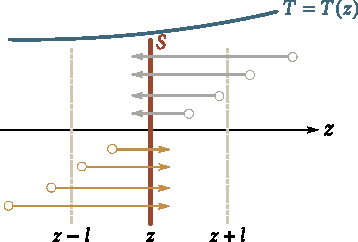
\includegraphics[scale=1]{figures/ch_16/fig_16_7.pdf}
		\caption[]{}
		\label{fig:16_7}
	\end{center}
	\vspace{-0.8cm}
\end{figure}

On the basis of simplified notions, we shall consider that the number of mole-cules flying in one second through area $S$ in each direction (from left to right and from right to left) is
\begin{equation}\label{eq:16_20}
    N = \frac{1}{6} n \average{v} S.
\end{equation}

At constant pressure, $n$ depends on the temperature ($p=nkT$), and $\average{v}$ also changes with the temperature. Accordingly, it would seem that to find the number of molecules flying through area $S$ from left to right we ought to use in \eqn{16_20} the values of $n$ and $\average{v}$ corresponding to one temperature, and to find the number of molecules flying from right to left, the values of $n$ and $\average{v}$ corresponding to another temperature. The numbers of molecules flying through area $S$ in opposite directions cannot differ, however. If they did, then apart from the heat flux through area $S$, we would also observe a flow of matter---the gas would be transported from one part of space to another. But we assumed that no processes occur in the gas except for the transport of heat. Therefore, we shall use \eqn{16_20} to calculate the number of molecules flying through $S$ in each direction, assuming for $n$ and $\average{v}$ their values in section $S$.

It must be noted that since $n=p/kT$, \ie, $n$ is proportional to $p/T$, and $\average{v}$ is proportional to $\sqrt{T}$, the constancy of the product $n\average{v}$ signifies the constancy of the expression
\begin{equation*}
    \frac{p}{T}\sqrt{T} = \frac{p}{\sqrt{T}}.
\end{equation*}

\noindent
Hence, for no flow of molecules to be observed when a temperature gradient is present, it is essential that the pressure change along the $z$-axis in proportion to $\sqrt{T}$.

In calculating the heat flux, we shall proceed from the assumption that every molecule carries with it the energy $\varepsilon=kT/2$ corresponding to the temperature at the spot where its last collision with another molecule occurred. On the average, this collision occurs at a distance from $S$ equal to the mean free path $l$ (see \fig{16_7}). Thus, the energy $\average{\varepsilon_1}$ corresponding to the temperature $T_1=T(z-l)$, \ie, to the temperature in the plane $(z-l)$, should be ascribed to the molecules flying in the direction of the $z$-axis, and the energy $\average{\varepsilon_2}$ corresponding to the temperature $T_2=T(z+l)$ should be ascribed to the molecules flying in the opposite direction (here $z$ is the coordinate of plane $S$).

In accordance with the above, we get the following expression for the heat flux through area $S$ in the positive direction of the $z$-axis:
\begin{equation*}
    q = N\parenthesis{\average{\varepsilon_1} - \average{\varepsilon_2}}
\end{equation*}

\noindent
where $N$ is determined by \eqn{16_20}. Introduction of the values of $N$, $\average{\varepsilon_1}$, and $\average{\varepsilon_2}$ yields
\begin{equation}\label{eq:16_21}
    q = \frac{1}{6} n\average{v} S \parenthesis{\frac{i}{2}kT_1 - \frac{i}{2}kT_2} = \frac{1}{6} n\average{v} S \frac{i}{2} k\parenthesis{T_1-T_2}.
\end{equation}

\noindent
The difference $T_1-T_2$ equals
\begin{equation}\label{eq:16_22}
    T (z-l) + T (z+l) = -\diff{T}{z} 2l
\end{equation}

\noindent
(we have taken into account the smallness of $l$). Here $\diffin{T}{z}$ is the derivative of $T$ with respect to $z$ at the location of plane $S$.

With a view to \eqn{16_22}, we can write \eqn{16_21} as follows:
\begin{equation}\label{eq:16_23}
    q = -\frac{1}{6} n\average{v} S \frac{i}{2}k\,\diff{T}{z} 2l = -\frac{1}{3} \average{v} l \parenthesis{\frac{i}{2}kn}\,\diff{T}{z} S.
\end{equation}

\noindent
A comparison of this equation with \eqn{16_3} gives the following expression for the thermal conductivity coefficient:
\begin{equation}\label{eq:16_24}
    \varkappa = \frac{1}{3} \average{v} l \parenthesis{\frac{i}{2}kn}.
\end{equation}

It should be remembered that the expression $iR/2=ik\ab{N}{A}/2$ determines the heat capacity at constant volume $C_V$ of one mole of a gas, \ie, the amount of a gas containing $\ab{N}{A}$ molecules. Similarly, the expression $ikn/2$ is the heat capacity of the amount of a gas containing $n$ molecules, \ie, the heat capacity of a unit volume of the gas. We can obtain this heat capacity by multiplying the specific
heat capacity $c_V$ (the heat capacity of a unit mass) by the mass of a unit volume, \ie, by the density of the gas $\rho$. Thus,
\begin{equation}\label{eq:16_25}
    \frac{i}{2}kn = \rho c_V.
\end{equation}

Introducing \eqn{16_25} into~\eqref{eq:16_24}, we arrive at the final expression for the thermal conductivity coefficient of a gas:
\begin{equation}\label{eq:16_26}
    \varkappa = \frac{1}{3} \average{v} l \rho c_V.
\end{equation}

\noindent
As we have expected, the thermal conductivity coefficient was found to be proportional to $\average{v}, l$, and the heat capacity of a gas $\rho c_V$. More strict calculations lead to a similar expression for $\varkappa$, but with a somewhat different numerical factor.

Let us find how $\varkappa$ depends on the quantities characterizing molecules and on the parameters of state of a gas. Taking into account that $average{v}$ is proportional to $\sqrt{T/m}$, $l$ is proportional to $1/n\sigma$, and $\rho c_V$ is proportional to $in$ [see \eqn{16_25}], we get
\begin{equation}\label{eq:16_27}
    \varkappa \propto \parenthesis{\frac{T}{m}}^{1/2} \frac{1}{n\sigma} i n = \frac{i}{\sigma} \parenthesis{\frac{T}{m}}^{1/2}.
\end{equation}

Inspection of expression~\eqref{eq:16_27} shows that unlike the diffusion coefficient, the thermal conductivity coefficient of a gas does not depend on the number of molecules in a unit volume, and, therefore, on the pressure ($p=nkT$). This is due to the following reasons. Reduction of the pressure is attended by diminishing of $n$, \ie, of the number of molecules participating in the transfer of energy. Simultaneously, $l$ grows and, consequently, also the difference between the energies transported by every molecule in opposite directions. As a result, we see that the amount of energy transferred by the molecules at the given temperature gradient does not depend on the pressure. This holds only as long as $l$ remains small in comparison with the distance between the surfaces exchanging heat at the expense of the thermal conductivity of the gas contained between them (for example, in comparison with the size of the gap between the internal and external walls of a glass vacuum bottle). As this condition stops being observed, the thermal conductivity begins to depend to a greater and greater extent on the pressure, diminishing when the latter lowers. When $l$ exceeds the distance between the surfaces, the path of the molecules is determined by the magnitude of this distance and stops depending on the pressure. The number of molecules per unit volume continues to fall off with decreasing pressure, the result being a reduction in $\varkappa$.

When the temperature is raised, the thermal conductivity coefficient grows somewhat more rapidly than $\sqrt{T}$. The cause is that the effective section a depends slightly on $T$ (see \sect{16_2}).

\section{Viscosity of Gases}\label{sec:16_5}

To understand the origin of forces of internal friction, let us consider two contacting layers of a gas having a thickness of $\Delta z$. We shall
assume that the layers move with different velocities $u_1$ and $u_2$ (\fig{16_8}). Every molecule of the gas participates in two motions: chaotic thermal motion whose mean velocity is $\average{v}$, and ordered motion with the velocity $u$ that is much smaller than $\average{v}$.

\begin{figure}[t]
	\begin{center}
		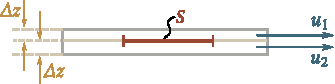
\includegraphics[scale=1]{figures/ch_16/fig_16_8.pdf}
		\caption[]{}
		\label{fig:16_8}
	\end{center}
	\vspace{-0.8cm}
\end{figure}

Suppose that at a certain moment the layers have the momenta $K_1$ and $K_2$. These momenta cannot remain unchanged because owing to thermal motion the continuous transition of molecules from one layer to another occurs. According to our simplified notions, the number of molecules passing through area $S$ from one layer to another a second is determined by the expression
\begin{equation}\label{eq:16_28}
    N = \frac{1}{6} n \average{v} S
\end{equation}

\noindent
(the insignificant effect of ordered motion on the magnitude of the velocity of the molecules may be disregarded). Upon getting into another layer, a molecule collides with the molecules of that layer. As a result, it either gives up its surplus momentum to other molecules (if it arrived from a layer moving with a greater velocity), or increases its momentum at the expense of the other molecules (if it arrived from a layer moving with a smaller velocity). As a result, the momentum of the faster layer diminishes, and of the slower one grows. The layers thus behave as if a retarding force is applied to the first layer (whose velocity is greater), and an accelerating force equal in magnitude is applied to the second layer (whose velocity is lower).

The momentum transferred through area $S$ on the interface between the layers depicted in \fig{16_8} in unit time from the first layer to the second one is
\begin{equation*}
    K = N \parenthesis{mu_1 - mu_2}
\end{equation*}

\noindent
($m$ is the mass of a molecule). Introduction of \eqn{16_28} for $N$
yields
\begin{equation}\label{eq:16_29}
    K = \frac{1}{6} n \average{v} S m \parenthesis{mu_1 - mu_2}.
\end{equation}

In a real gas flow, the velocity when crossing the interface between two layers changes not in a jump, but continuously according to the law $u=u(z)$ (\fig{16_9}). We shall consider that every molecule flying through surface $S$ carries along with it the momentum $mu$ determined by the value of the velocity $u$ at the spot where the last collision of
the molecule occurred. Different molecules experience their last collision at the most diverse distances from $S$. On the average, this collision occurs at a distance equal to the free path $l$. We shall therefore ascribe the velocity $u_1=u(z-l)$ to the molecules flying in the direction of the $z$-axis, and the velocity $u_2=u(z+l)$ to the molecules flying in the opposite direction. Inserting these values in \eqn{16_29}, we get the following expression for the momentum flux in the direction of the $z$-axis:
\begin{equation*}
    K = \frac{1}{6} n \average{v} S m \bracket{u(z-l)-u(z+l)} = \frac{1}{6} n \average{v} S m\,\diff{u}{z} 2l
\end{equation*}

\noindent
[compare with \eqn{16_23}].

\begin{figure}[t]
	\begin{center}
		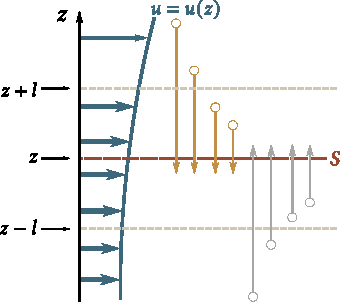
\includegraphics[scale=1]{figures/ch_16/fig_16_9.pdf}
		\caption[]{}
		\label{fig:16_9}
	\end{center}
	\vspace{-0.8cm}
\end{figure}

Taking into account that the product nm equals the density of a gas $\rho$, we can write that
\begin{equation*}
    K = -\parenthesis{\frac{1}{3} \average{v} l \rho}\,\diff{u}{z} S.
\end{equation*}

\noindent
A comparison with \eqn{16_5} gives an expression for the viscosity:
\begin{equation}\label{eq:16_30}
    \eta = \frac{1}{3} \average{v} l \rho.
\end{equation}

\noindent
Stricter calculations lead to the same expression, but with a somewhat different numerical factor.

It can he seen from \eqn{16_30} that like $D$ and $\varkappa$, the viscosity is proportional to $\average{v}$ and $l$. It is also proportional to the density of a gas $\rho$, \ie, to a quantity characterizing the ability of a gas to ``accumulate'' momentum---at a given velocity $u$ the momentum of a unit volume of a gas is the greater, the higher is the density $\rho$ (we remind our reader that the thermal conductivity is proportional to the heat capacity of a unit volume of a gas).

Taking into account the expressions for the quantities in \eqn{16_30}, we can write that
\begin{equation*}
    \eta \propto \parenthesis{\frac{T}{m}}^{1/2} \frac{1}{n\sigma} n m = \frac{\sqrt{mT}}{\sigma}.
\end{equation*}

\noindent
Hence, it follows that like $\varkappa$, the viscosity does not depend on the pressure. This holds only as long as $l$ remains small in comparison with the size of the gap through which the gas is flowing (for example, in comparison with the diameter of a pipe). As this condition stops being observed, the viscosity begins to depend more and more on the pressure, diminishing when the latter drops. The viscosity $\eta$ depends on the temperature in the same way as $D$ and $\varkappa$.

\section{Ultrararefied Gases}\label{sec:16_6}

When the free path of molecules exceeds the linear dimensions of the vessel confining them, we say that a vacuum has been achieved in the vessel. The gas in this case is called \textbf{ultrararefied}. Although the word vacuum literally means ``emptiness'', an ultrararefied gas contains a great number of molecules in a unit volume. Thus, at a pressure of \SI{e-6}{\mmHg}, one cubic metre contains about \num{e16} molecules. Moreover, in very minute pores, the state defined as a vacuum can also be achieved at atmospheric pressure.

The behaviour of ultrararefied gases is distinguished by numerous features. For conditions of a vacuum, we cannot speak of the pressure of one part of a gas on another. In ordinary conditions, the molecules often collide with one another. Consequently, any surface with which we mentally divide a gas into two parts will experience an exchange of momenta between molecules. Thus, one part of the gas will act on the other with the pressure $p$ over the interface. In a vacuum, the molecules exchange momenta only with the wa1ls of the vessel, so that only the concept of the pressure of a gas on a wall has a meaning. Internal friction is also absent in the gas. But a body moving in an ultrararefied gas will experience the action of a friction force due to the fact that the molecules colliding with this body will change its momentum. Let us consider this in greater detail.

Assume that two plates are moving parallel to each other in an ultrararefied gas (\fig{16_10}). The velocities of the plates are $u_1$ and $u_2$. The interaction between a molecule and a plate at the moment of a collision leads to the molecule, upon rebounding from the plate, having a velocity component equal in magnitude and direction to the velocity of the plate in addition to its thermal velocity.

A unit area of the upper plate will be struck in one second by $n\average{v}/6$ molecules having a velocity component $u_2$ acquired in the preceding collision with the lower plate. Each of these molecules carries a momentum component of $mu_2$. Upon rebounding from the upper plate, the molecules have a momentum component of $mu_1$.

Consequently, a collision of every molecule with the upper plate results in its momentum diminishing by $m\parenthesis{u_1-u_2}$. The change in the momentum in unit time related to unit surface area of the plate is
\begin{equation*}
    \frac{1}{6} n \average{v} m \parenthesis{u_1-u_2}.
\end{equation*}

\noindent
This change equals the force acting on a unit surface area of the plate:
\begin{equation}\label{eq:16_31}
    F = \frac{1}{6} \rho \average{v} \parenthesis{u_1-u_2}
\end{equation}

\noindent
(we have substituted $p$ for $nm$). A force of the same magnitude, but opposite in direction, acts on a unit surface area of the lower plate.

It is natural to call the proportionality constant between the force of friction and the velocity difference of the plates the coefficient of friction. It can be seen from \eqn{16_31} that this coefficient equals $\rho\average{v}/6$, \ie, is proportional to the density of the gas and, consequently, to the pressure of the gas on a plate and the walls of the vessel (the expression $p=nkT$ remains in force for this pressure).

\begin{figure}[t]
	\begin{minipage}[t]{0.5\linewidth}
		\begin{center}
			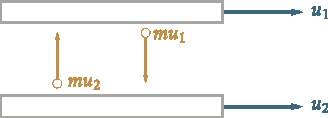
\includegraphics[scale=1]{figures/ch_16/fig_16_10.pdf}
			\caption[]{}
			\label{fig:16_10}
		\end{center}
	\end{minipage}
	\hspace{-0.05cm}
	\begin{minipage}[t]{0.5\linewidth}
		\begin{center}
			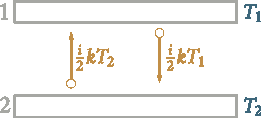
\includegraphics[scale=1]{figures/ch_16/fig_16_11.pdf}
			\caption[]{}
			\label{fig:16_11}
		\end{center}
	\end{minipage}
	\vspace{-0.4cm}
\end{figure}

Let us now consider the transfer of heat by a gas in a vacuum. We shall consider two plates with temperatures $T_1$ and $T_2$ between which there is an ultrararefied gas (\fig{16_11}). If the impact of the molecules against the surface of the rigid body were of a perfectly elastic nature, the molecules would rebound from a plate with the same velocity in magnitude (and, consequently, with the same energy) as they had before the collision. As a result, the molecules would not be able to transfer energy from one plate to the other. Such a conclusion, however, contradicts experimental data. Hence, the interaction between a wall and a molecule striking it is not an elastic collision in nature. Indeed, it occurs as follows: upon striking a wall, a molecule adheres to it, as it were, for a brief time, after which it leaves the wall in an absolutely arbitrary direction with a velocity whose magnitude on the average corresponds to the temperature of the wall\footnote{We must note that this more precise definition of the nature of interaction of the molecules with a wall does not affect the results which we obtained in \sect{11_4} when calculating the pressure. If the temperature of the gas and the walls is the same, then the molecules will leave a wall with the same mean velocity with which they collided with it, so that the change in the momentum of the molecules as a result of a collision is the same on an average as in a perfectly elastic collision.}.

Let us revert to \fig{16_11}. Each of the $n\average{v}S/6$ molecules striking the upper plate a second carries the energy $ikT_2/2$ along with
it and carries away an energy of $ikT_1/2$. Hence, each impact of a molecule against a plate leads to the latter losing the energy $ik\parenthesis{T_1-T_2}/2$. The second plate receives the same energy upon each impact. Thus, the amount of energy transferred by the molecules in one second from plate to plate will be
\begin{equation*}
    q = \frac{1}{6} n \average{v} \frac{i}{2} k \parenthesis{T_1-T_2} S.
\end{equation*}

\noindent
Multiplying and dividing this expression by $m\ab{N}{A}$, we get
\begin{equation}\label{eq:16_32}
    q = \frac{1}{6} \rho \average{v} c_V \parenthesis{T_1-T_2} S.
\end{equation}

The thermal conductivity coefficient equal to $\rho\average{v}c_V/6$ is found to be proportional to the density of a gas when the latter is ultrararefied. Hence, heat transfer from one wall to another will fall off with decreasing pressure, whereas the thermal conductivity of a gas in ordinary conditions does not depend, as we have seen, on the pressure.
